\documentclass{beamer}

\title{Pushouts in topological spaces}
\author{Ruth Plümer}
\institute{Practical training course: Formalizing mathematics in Lean}
\date{\today}
\usetheme{Madrid}
\usepackage{url}
\usepackage{tikz-cd}
\usetikzlibrary{cd}

\begin{document}
	\begin{frame}
		\titlepage 
	\end{frame}
	% Outline frame
	\begin{frame}{Outline}
		\tableofcontents
	\end{frame}
	% Presentation structure
	\section{Mathematical background}
	\subsection{Definition of the adjunction space}
	\subsection{Universal properties}
	\subsection{Interesting lemmas}
	\section{Formalization}
	\subsection{Implementing the definition}
	\subsection{Challenging aspects}
	\section{Future work?}
	\begin{frame}
		\frametitle{Mathematical background}
		\framesubtitle{Definition of the adjunction space}
		\begin{definition}
			Let $X$ and $Y$ be topological spaces, $X \sqcup Y$ be the disjoint union and $\varphi_1 : X \to X \sqcup Y$ and $\varphi_2 : Y \to X \sqcup Y$ be the canonical inclusion maps. The topology $\mathcal{O}$ on $X \sqcup Y$ is given by
			$$ \mathcal{O} := \{ U \subseteq X \sqcup Y \, \vert \, \varphi_1^{-1}(U) \text{ is open in } X \text{ or } \varphi_2^{-1}(U) \text{ is open in }Y \}. $$
		\end{definition}
		\begin{definition}
			Let $X$ be a topological space and $\sim$ be an equivalence relation on $X$. Then, the \textbf{quotient space} $X /_{\sim}$ is the set $\{[x] : x \in X\}$ of equivalence classes together with the topology 
			$$\mathcal{O} := \{U \subseteq X /_{\sim} \, \vert \, \exists V \subseteq X \text{ open} : x \in V \Leftrightarrow [x] \in U\}.$$
		\end{definition}
	\end{frame}
	\begin{frame}
		\frametitle{Mathematical background}
		\framesubtitle{Definition of the adjunction space}
		\begin{definition}
			Let $X$ and $Y$ be topological spaces and let $A$ be a subspace of $Y$. Moreover, let $f_1 : A \to X$ be continuous and $f_2 : A \to Y$ be the inclusion map. \\
			Moreover, let $\sim$ be the equivalence relation on $X \sqcup Y$ generated by $f_1(a) \sim f_2(a)$ for all $a \in A$. Then, the quotient 
			$$X \cup_{f_1} Y := (X \sqcup Y) /_{\sim}$$
			with the quotient topology is called the adjunction space (or pushout).
		\end{definition}
	\end{frame}
	\begin{frame}[fragile]
		\frametitle{Mathematical background}
		\framesubtitle{Universal properties}
		\begin{theorem}[Universal property of the disjoint union]
			Let $X, Y, Z$ be topological spaces and $f_1 : X \to Z$ and $f_2 : Y \to Z$ be continuous maps. Then there exists exactly one continuous map $g : X \sqcup Y \to Z$ with $f_1 = g \circ \varphi_1$ and $f_2 = g \circ \varphi_2$.
		\end{theorem}
		\begin{tikzcd}[row sep=huge]
			& Z  & \\
			X\ar[ur,"f_1",sloped] \ar[r,"\varphi_1", swap] & X\sqcup Y \ar[u,dashed,"{g}" description] & Y \ar[ul,"f_2", swap,sloped] \ar[l,"\varphi_2"]
		\end{tikzcd}
		
		The disjoint union is the coproduct in the category of topological spaces.
	\end{frame}
	\begin{frame}[fragile]
		\frametitle{Mathematical background}
		\framesubtitle{Universal properties}
		\begin{theorem}[Universal property of the quotient space]
			Let $X, Z$ be topological spaces, $\sim$ be an equivalence relation on $X$ and $f : X \to Z$ be continuous with $x_1 \sim x_2 \Rightarrow f(x_1) = f(x_2)$. Then there exists exactly one continuous map $g : (X /_{\sim}) \to Y$ with $g([x]) = f(x)$ for all $x \in X$. 
		\end{theorem}
		\begin{tikzcd}
			X \arrow[r] \arrow[dr, "f"]
			& X /_{\sim} \arrow[d, dashed, "g"]\\
			& Y
		\end{tikzcd}
	\end{frame}
	\begin{frame}[fragile]
		\frametitle{Mathematical background}
		\framesubtitle{Universal properties}
		\begin{theorem}[Universal property of the pushout]
			Let $X, Y, Z$ be topological spaces, $A$ a subspace of $Y$, $f_1 : A \to X$ be continuous and $f_2 : A \to Y$ be the inclusion map.\\
			Moreover, let $g_1 : X \to Z$ and $g_2 : Y \to Z$ be continuous maps with $g_1 \circ f_1 = g_2 \circ f_2$. \\
			Then there exists exactly one continuous map $h : X \cup_{f_1} Y \to Z$ with $g_1 = h \circ \varphi_1$ and $g_2 = h \circ \varphi_2$.
		\end{theorem}
	\begin{tikzcd}
		A \arrow[d,"f_1"'] \arrow[r,hook,"f_2"] &
		Y \arrow[d,"\varphi_2"'] \arrow[ddr,bend left,"g_2"] \\
		X \arrow[r,"\varphi_1"] \arrow[drr,bend right,"g_1"'] &
		X \cup_{f_1} Y \arrow[dr,dashed,"h"] \\
		&& Y
	\end{tikzcd}
	\end{frame}
	\begin{frame}
		\frametitle{Mathematical background}
		\framesubtitle{Interesting lemmas}
		\begin{lemma}
			$\varphi_1$ is an embedding.
		\end{lemma}
		\pause[2]
		\begin{lemma}
			If $A$ is closed in $X$, $\varphi_1$ is a closed embedding.
		\end{lemma}
		\pause[3]
		\begin{lemma}
			If $A$ is closed in $X$, $\varphi_2 \vert_{Y \setminus A}$ is an open embedding.
		\end{lemma}
		\pause[4]
		\begin{lemma}
			If $f_1$ is a quotient map, $\varphi_2$ is a quotient map as well.
		\end{lemma}
	\end{frame}
	\begin{frame}
		\frametitle{Mathematical background}
		\framesubtitle{Interesting lemmas}
		\begin{definition}[Connectedness]
			A topological space $X$ is called \textbf{connected} if and only if the only subsets of $X$ that are both open and closed are $\emptyset$ and $X$.
		\end{definition}
		\pause[2]
		\begin{definition}[Path-connectedness]
			A topological space $X$ is called \textbf{path-connected} if and only if for all $x, y \in X$ there exists a continuous map $p : [0,1] \to X$ with $p(0) = x$ and $p(1) = y$.
		\end{definition}
		\pause[3]
		\begin{lemma}
			If $A$ is nonempty and $X$ and $Y$ are connected, $X \cup_{f_1} Y$ is connected as well.
		\end{lemma}
		\pause[4]
		\begin{lemma}
			If $A$ is nonempty and $X$ and $Y$ are path connected, $X \cup_{f_2} Y$ is path connected as well.
		\end{lemma}
	\end{frame}
	\begin{frame}
		\frametitle{Mathematical background}
		\framesubtitle{Interesting lemmas}
		\begin{definition}
			A nonempty topological space $X$ is called a \textbf{$T_1$-space} if and only if every set $S$ with $\left\vert S \right\vert = 1$ is closed.
		\end{definition}
		\pause[2]
		\begin{lemma}
			Let $A$ be closed in $Y$ and $X$ and $Y$ be $T_1$-spaces. Then $X \cup_{f_1} Y$ is a $T_1$-space as well.
		\end{lemma}
	\end{frame}
	\begin{frame}
		\frametitle{Mathematical background}
		\framesubtitle{Interesting lemmas}
		\begin{definition}[Normal space]
			A topological space $X$ is called \textbf{normal} if and only if for all disjoint closed sets $C, D \subseteq X$ there exist disjoint open sets $U, V \subseteq X$ with $C \subseteq U$ and $D \subseteq V$.
		\end{definition}
		\pause[2]
		\begin{definition}[T4 space]
			A nonempty topological space $X$ is called \textbf{$T_4$-space} iff it is both $T_1$ and normal.
		\end{definition}
		\pause[3]
		\begin{theorem}[Tietze's extension theorem]
			Let $X$ be a normal space, $C \subseteq X$ closed and $f : C \to \mathbb{R}$ be a continuous map. Then there exists a continuous map $f' : X \to \mathbb{R}$ with $f'\vert_{C} = f$.
		\end{theorem}
	\end{frame}
	\begin{frame}
		\frametitle{Mathematical background}
		\framesubtitle{Interesting lemmas}
		\begin{lemma}
			Let $X, Y$ be $T_4$-spaces, $A \subseteq Y$ a nonempty closed subspace of $Y$, $f_1 : A \to X$ be continuous and $f_2 : A \to Y$ be the inclusion map. Then $X \cup_{f_1} Y$ is a $T_4$-space as well.
		\end{lemma}
	\end{frame}
	\begin{frame}
		\frametitle{Formalization}
		\framesubtitle{Implementing the definition}
		Disjoint unions and quotient spaces are already implemented in mathlib as more general concepts:
		
		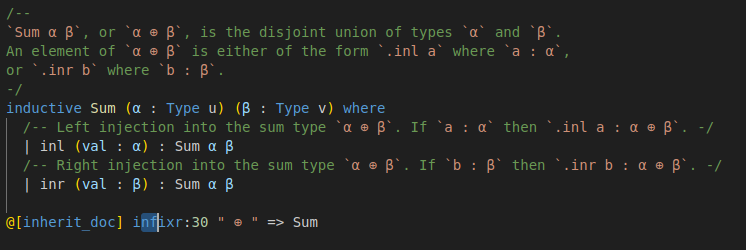
\includegraphics[width = 0.8\textwidth]{Disjoint_union.png}
		
		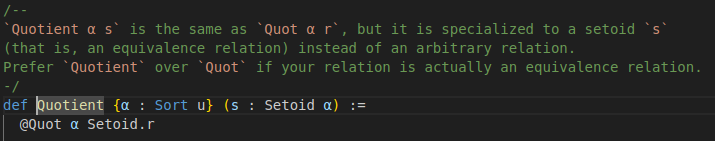
\includegraphics[width = 0.8\textwidth]{Quotient.png}
	\end{frame}
	\begin{frame}
		\frametitle{Formalization}
		\framesubtitle{Implementing the definition}
		The topologies on the disjoint union and the quotient space are given as instances of TopologicalSpace:
		
		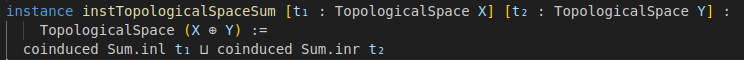
\includegraphics[width = 0.8\textwidth]{Disjoint_union_topology.png}
		
		\includegraphics[width = 0.8\textwidth]{Quotienttopology.png}
	\end{frame}
	\begin{frame}
		\frametitle{Formalization}
		\framesubtitle{Implementing the definition}
		Steps when implementing the definition of AdjunctionSpace:
		\begin{enumerate}
			\item Defining the equivalence relation on the disjoint union (equivalence\_of\_images $f_1$ $hf_2$)
			\item Defining $A$ and $Y$ as seperate types and defining the subspace relation by requiring $f_2$ to be an embedding.
		\end{enumerate}
	\end{frame}
\end{document}